% !TEX root =  paper.tex
\section{Background}\label{sec:background}

%In this section, we present basic concepts
%about E2E test automation that are needed 
%to understand the remainder of the paper.
%We provide background information on 
%DOM-based and visual web testing approaches.
%To present these approaches and concepts
%we use the example provided in~\autoref{fig:ab-back}: 
%a simplified version of the AddressBook web application, 
%one of the subjects used in our study. 
%We consider a scenario in which a user 
%inserts a \texttt{username} and \texttt{password} 
%in the AddressBook login form 
%(\autoref{fig:ab-back-a}), 
%and if these credentials are correct, 
%the \texttt{username} (\texttt{`admin'}) is displayed on the top right corner of the homepage 
%(\autoref{fig:ab-back-b}).

\noindent
\textbf{Approaches to E2E Web Test Automation.}
In recent years, two major approaches to E2E web testing have emerged, each of them characterized by a diverse way of interacting with the AUT. 

\textit{DOM-based} tools access and inspect properties of the Document Object Model (DOM), the hierarchical structure underlying a web page. 
%To this category belong capture-replay (C\&R) and programmable tools. \textit{Capture-replay} tools are based on the recording of sequences of inputs and actions performed by the tester on the web application GUI. The recording process creates a test script (see~\autoref{t:seleniumtest}) that can be replayed in a unattended mode. 
%With \textit{programmable} tools, on the other hand, test cases themselves become software artefacts that developers write resorting to specific testing frameworks (see~\autoref{lst:login-no-abs-back}). 
Specific testing framework APIs support the creation of test scripts that automate the interaction with a web page and its elements, and the sequences of inputs and actions performed by the tester on the web application. A test script can, for instance, automatically fill-in and submit forms or click on hyperlinks. %(see \autoref{fig:ab-back-c}). 
There are many test automation tools for web applications available, e.g., Selenium~\cite{selenium}, Sahi~\cite{sahi}, and Ringer~\cite{ringer}. %A representative of the programmable category is Selenium WebDriver~\cite{selenium}, which is considered the flagship open-source test automation tool for web applications.

An emerging and relatively new approach is \textit{visual} web testing, in which the AUT is tested through its GUI. 
%Indeed, the emergence of new complex visual components in web pages has required new ways of interfacing with the web applications. 
Visual tools such as JAutomate~\cite{Alegroth2013jat}, Sikuli~\cite{Sikuli}, and EggPlant Functional~\cite{eggplant} use image recognition techniques to identify the web elements displayed on the web page. Visual web testing tools offer an interesting alternative, and they are increasingly being adopted also in industry~\cite{Alegroth2013jat}. 
%\autoref{fig:ab-back-d} shows the visual version of the DOM-based test of~\autoref{fig:ab-back-c}, developed using Sikuli~\cite{Sikuli}. 
%We can notice how web elements are localised by \textit{visual locators}, i.e., images representing a portion of the GUI.

\noindent
\textbf{The Dilemma.}
To date, both approaches coexist and are utilized. Since each category of testing tools come with advantages and disadvantages, it is not clear whether in the future one will eventually prevail over the other. Our insight behind this uncertain scenario is that the choice of the most adequate testing tool depends to a large extent on the characteristics of the AUT. For instance, for highly-interactive web systems having complex visual components (e.g., Google Maps), the DOM can be complicated to retrieve, whereas relying on visual testing allows testers to more easily assert on the correctness of the web page visual content.
Additionally, most of popular DOM-based tools (e.g., Selenium) do not take into account the visual appearance of the AUT, which is instead important because it is tipically used by the tester as the main oracle against which to evaluate the correctness of the application. Visual tools, on the other hand, completely abstract away the model of the page, and create actions and assertions in a purely visual manner. 
%
Hybrid approaches such as Applitools~\cite{applitools} try to unify the two approaches and allow a tester to manually inject visual checks at specific places of the test execution. This has two drawbacks: (1)~the insertion of the check-points must be performed manually, (2)~this extra-code clutters the initial test code, with statements that do not pertain to the test scenario itself.

\noindent
\textbf{The Idea.}
We believe that the use of visual technologies in web testing can  be especially beneficial for regression testing purposes, rather than for test creation. For example, the GUI can be used to validate the correct execution of the tests as the AUT evolves over time (in a similar way as testers do), or to detect deviations from the correct behaviour.
Indeed, E2E tests are vastly used in \textit{regression} scenarios, i.e., to verify that the most recent code changes have not adversely affected existing features. To do so, already in place test cases are re-executed to ensure that the current functionalities still work correctly. 
%

\begin{figure*}[t]
\centering
\begin{subfigure}{\columnwidth}
\centering
%\fbox{
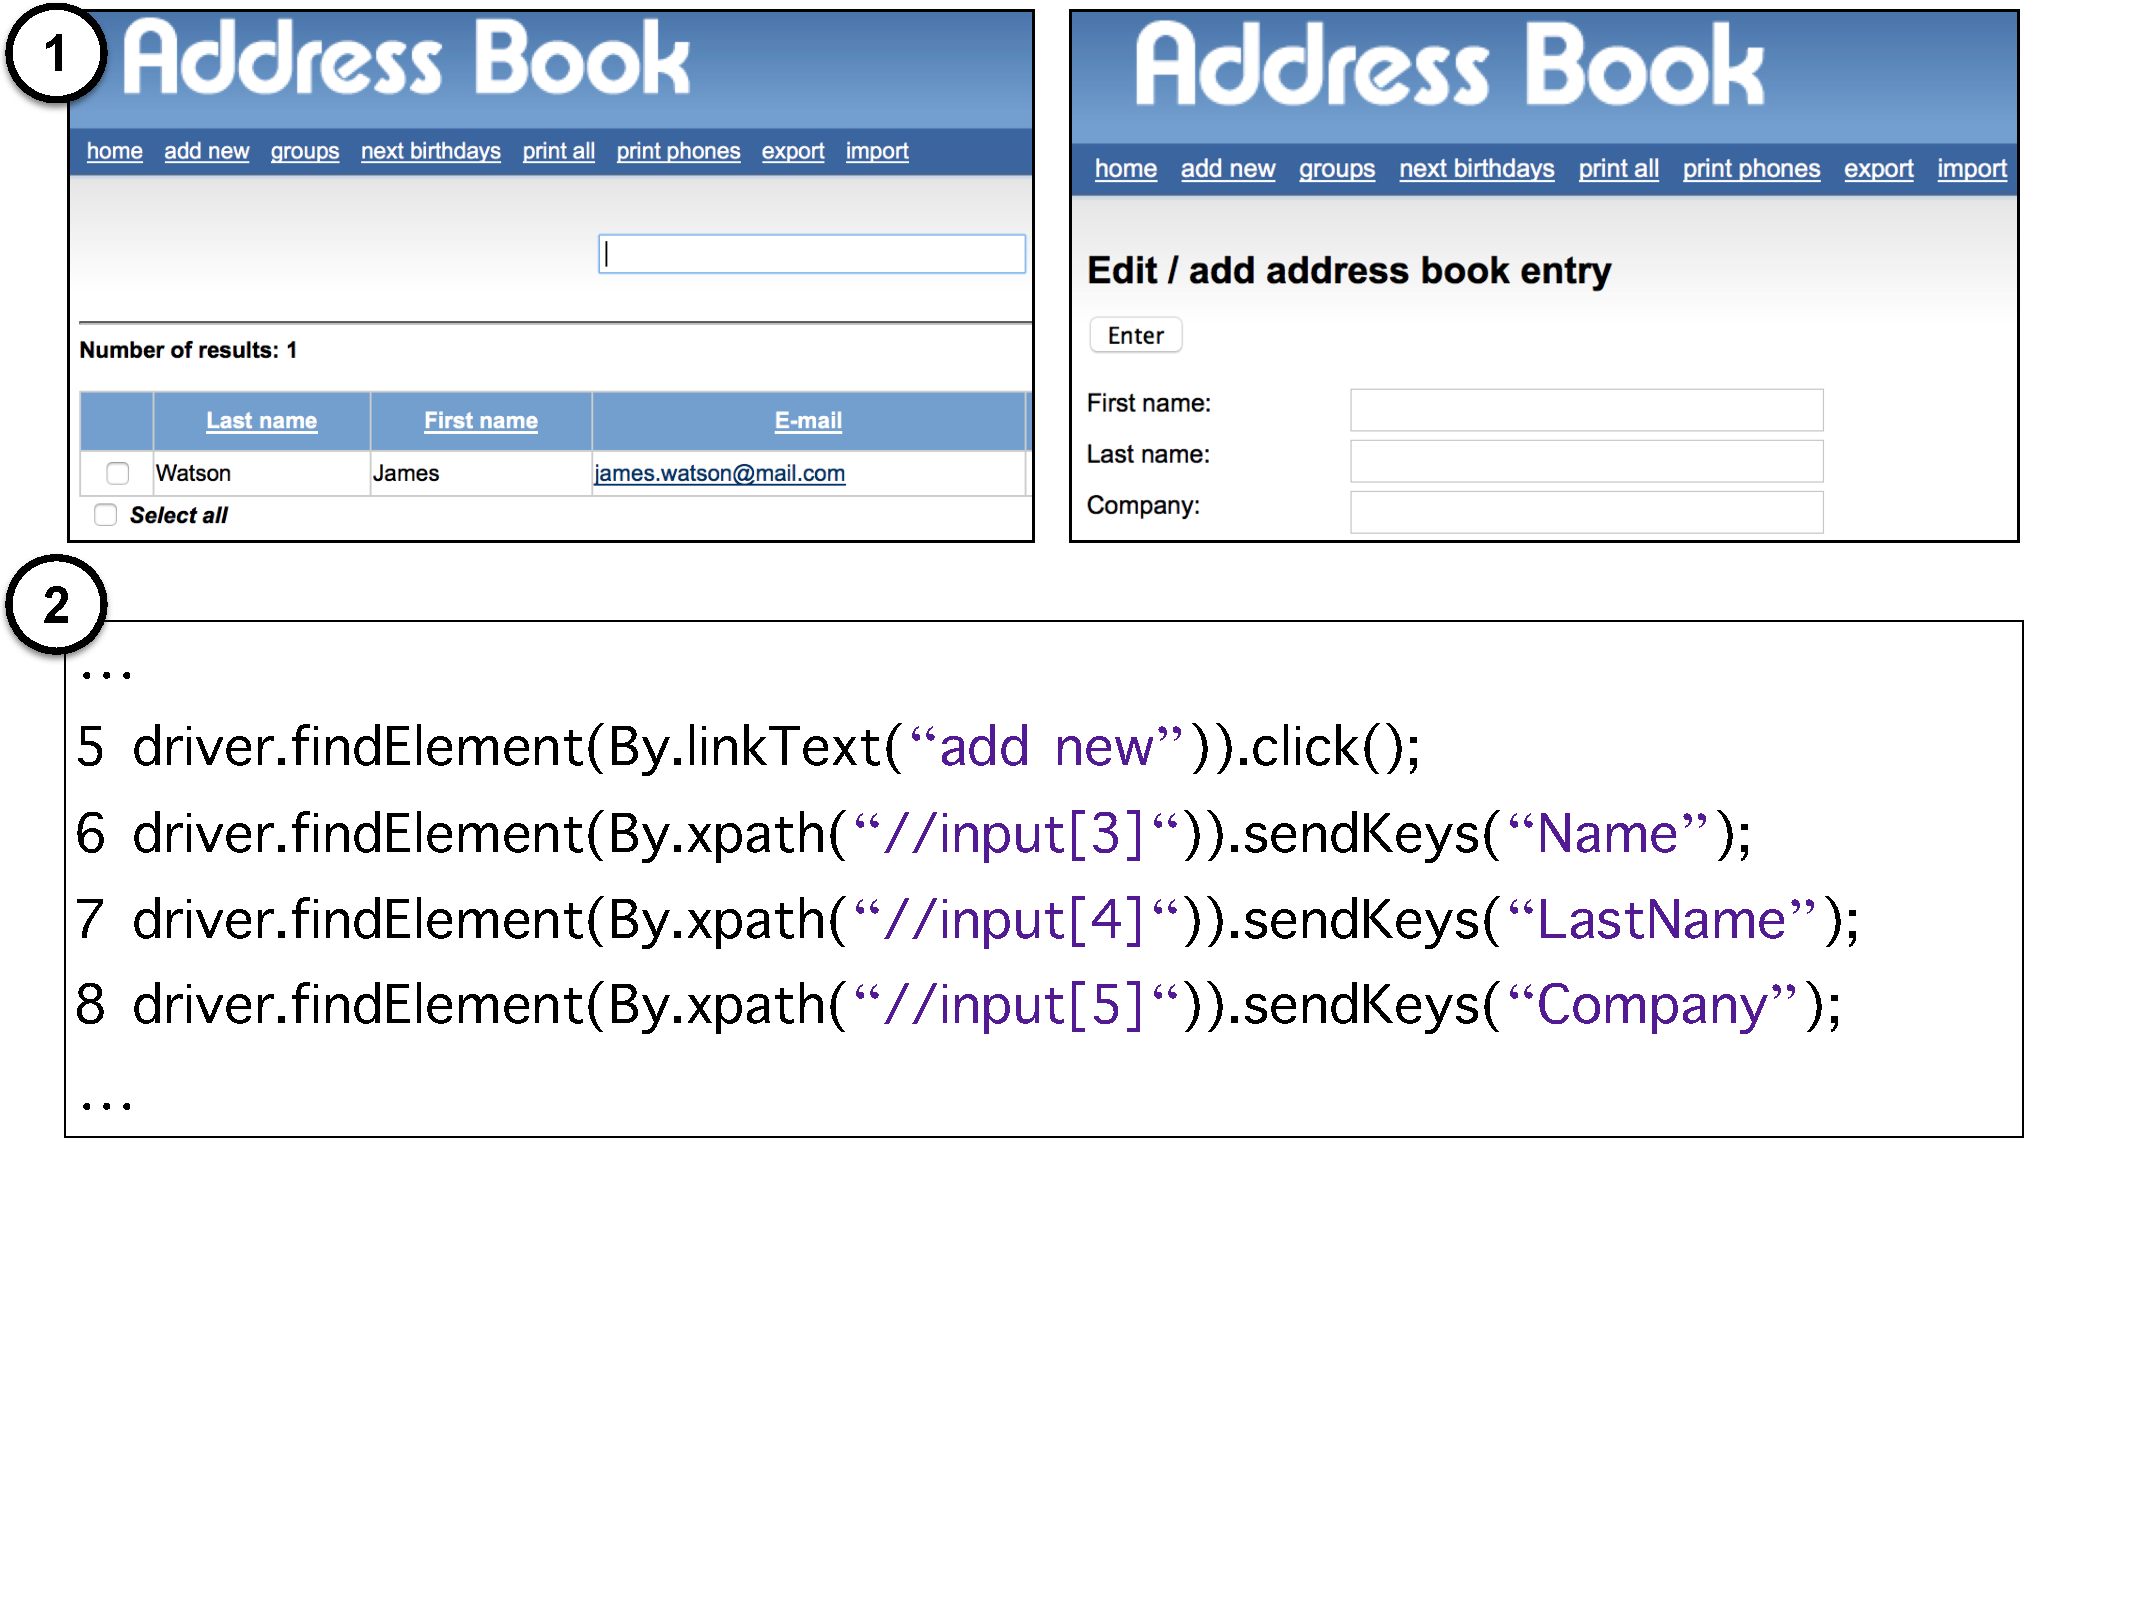
\includegraphics[trim=0cm 7.5cm 1.8cm 0cm, clip=true, scale=0.23]{images/addressbook-version1.pdf}
%}
\caption{\emph{Version 6.2.12}}
\label{fig:ab1} 
\end{subfigure}
\begin{subfigure}{\columnwidth}
\centering
%\fbox{
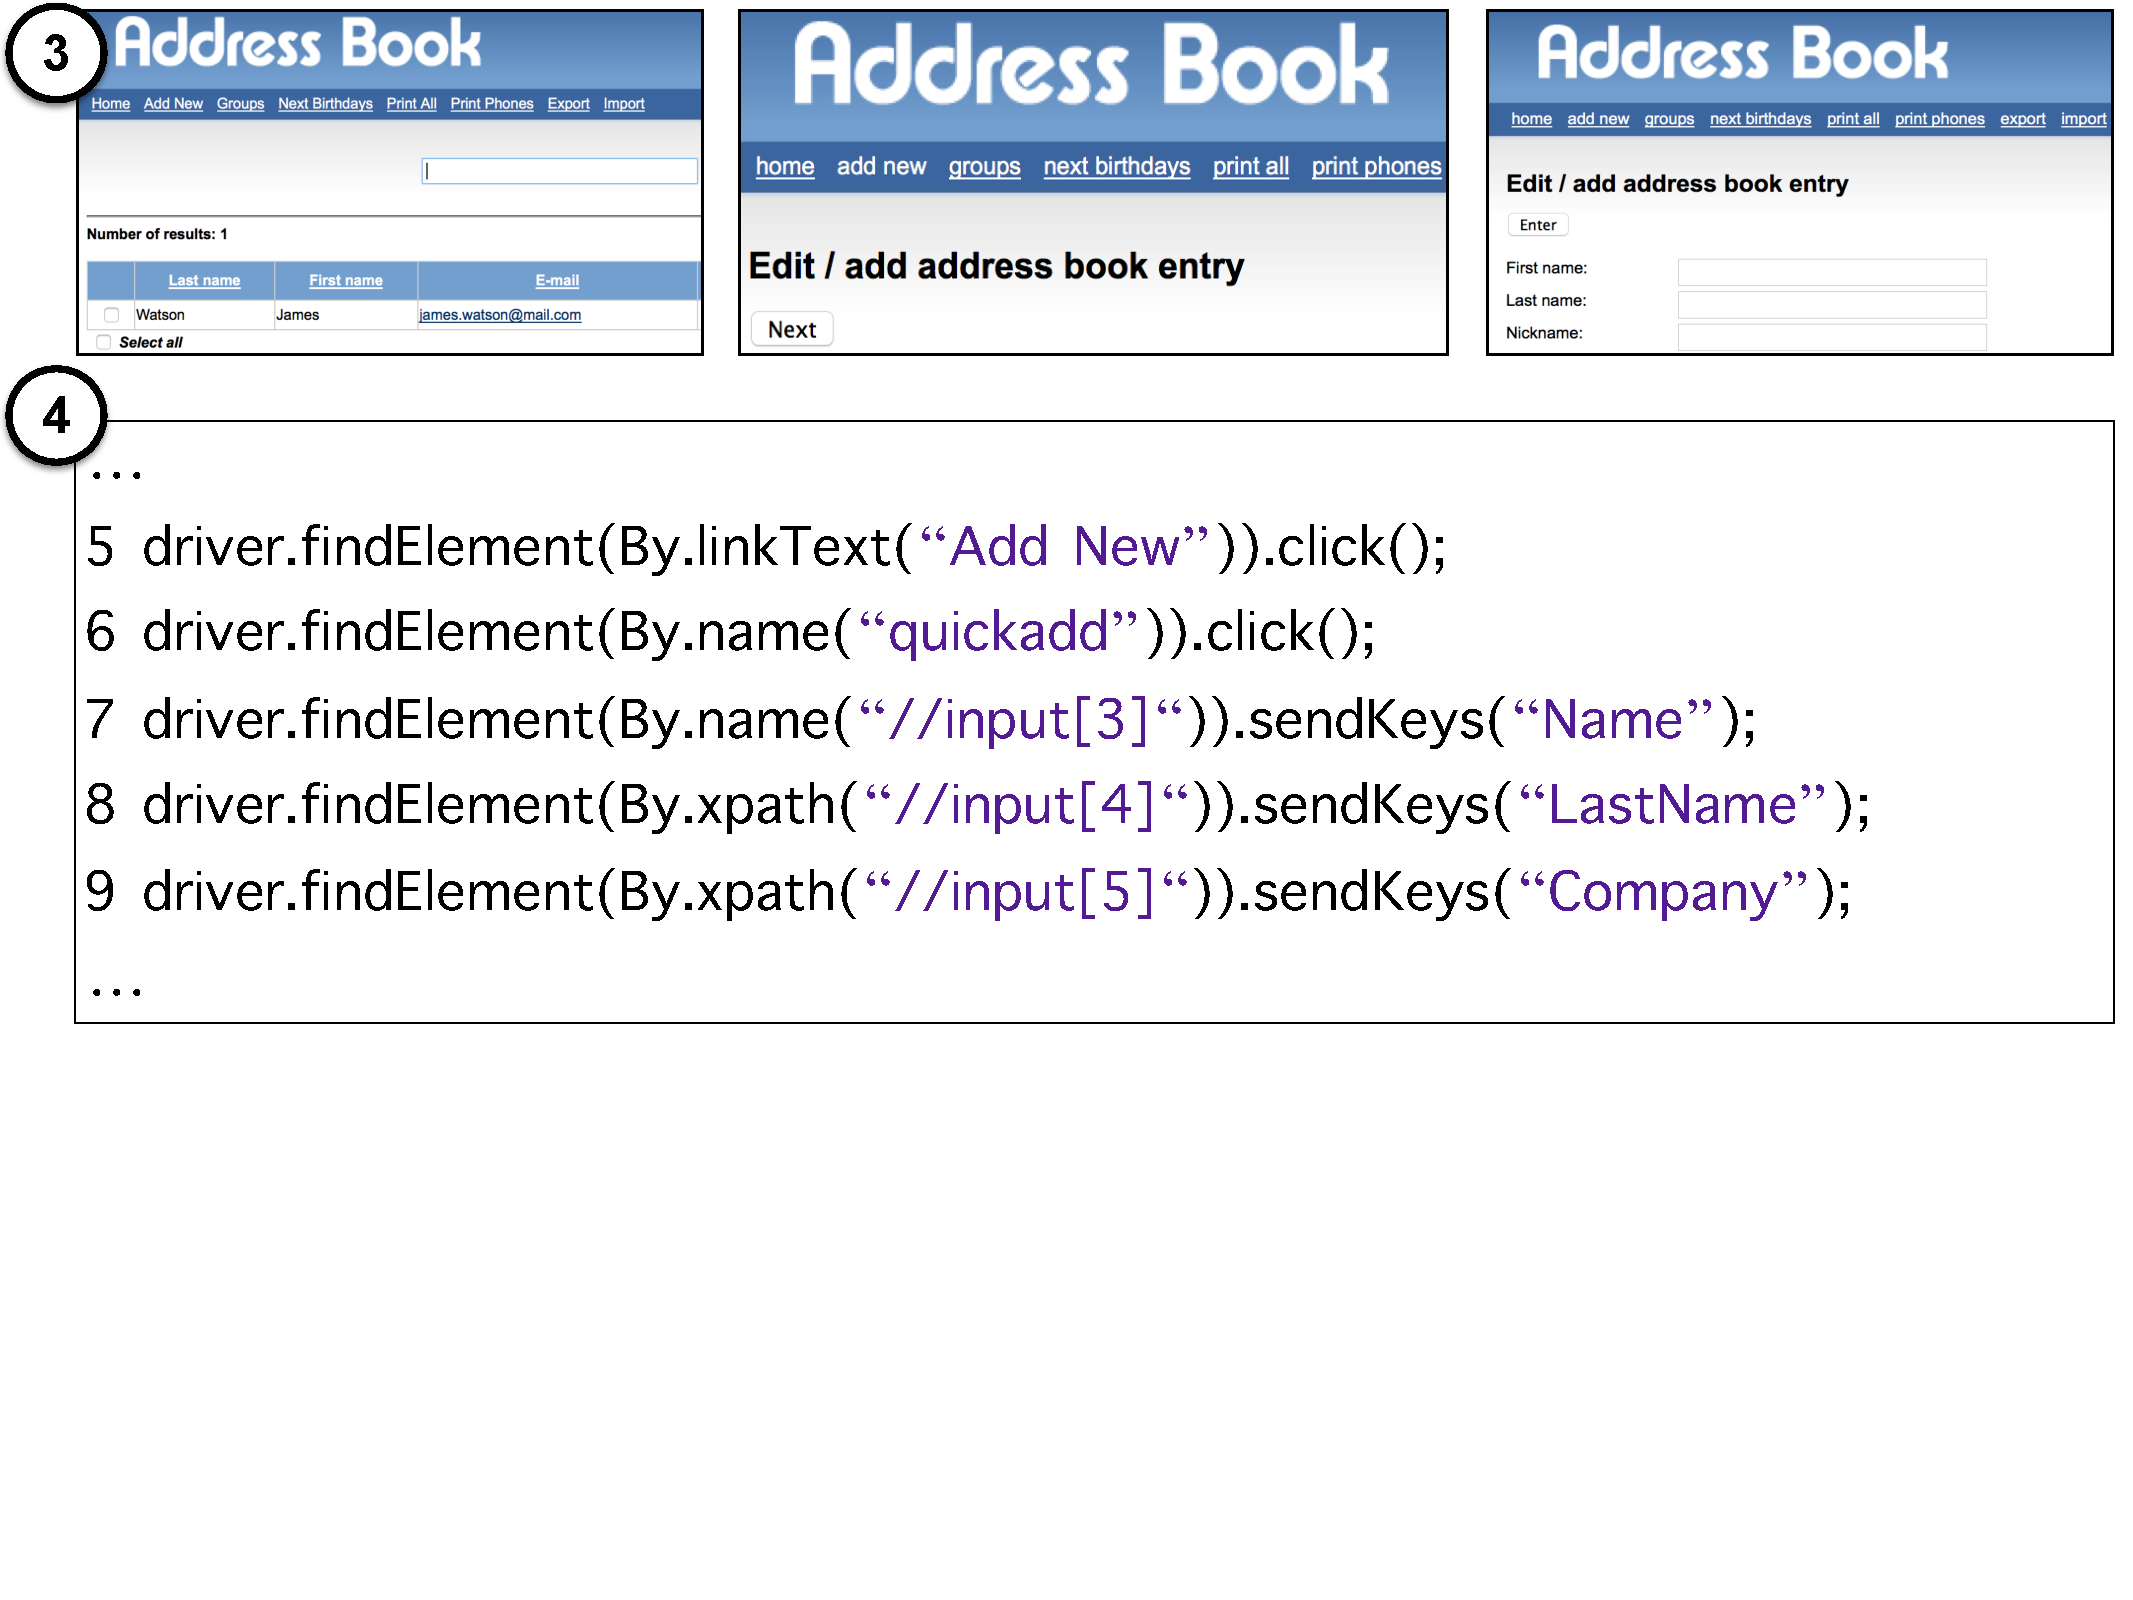
\includegraphics[trim=0cm 9.5cm 0cm 0cm, clip=true,  scale=0.260]{images/addressbook-version2.pdf}
%}
\caption{\emph{Version 7.0.0}}
\label{fig:ab2} 
\end{subfigure}
\caption{AddressBook web application, version 6.2.12 (\ref{fig:ab1}) and version 7.0.0 (\ref{fig:ab2}), along with  automated Selenium WebDriver tests. \andrea{find a way to show the web pages bigger}} 
\label{fig:example} 
\end{figure*}

\subsection{A Test Breakage Travelogue}\label{sec:breakage-travelogue}

Web tests are unfortunately known for being very fragile in the face of software evolution~\cite{2016-leotta-Advances,2016-Leotta-JSEP,Hammoudi-2016-ICST}. %Indeed, automated test code is usually highly coupled with low-level implementation details such as HTML attributes and thus result fragile and difficult to maintain as the AUT evolves~\cite{2016-leotta-Advances,2016-Leotta-JSEP,Hammoudi-2016-ICST}. 
Even a minor change might break a previously developed test case, whose script would need to be repaired manually, or re-written to match the new version of the web application, even if conceptually the functionality is unaltered, and no errors are present in the application code.

\noindent
\textbf{Characterization of a breakage.}
In order to clarify the scope of our work, and avoid possible misinterpretations, it is hence important to emphasize the difference between test breakages and test failures. We consider a \textit{test breakage} as the event that occur when a test that was used to work and pass on a certain version $V$, fails to be applicable to a version $V+n$ ($n \geq 1$) due to changes in the application code that interrupt its execution unpremeditatedly. %This event arises, for instance, when the test no longer reflects the intended behavior of the web application.
This is different from cases when tests expose a program \textit{failure} and hence do something for which they have been designed (i.e., exposing regression faults).
Said that, in the context of this paper, we focus our analysis on test breakages.

\noindent
\textbf{Study of Breakages.}
In a recent study, researchers have categorized breakages happening as test suites for web applications are evolved~\cite{Hammoudi-2016-ICST}. 
%While the study considers C\&R test suites only, the taxonomy of breakages proposed by Hammoudi and colleagues offers interesting findings. 
%
Concerning the \textit{causal} characterization, web element \textit{locators} have emerged as the main cause of fragility (74\% of the totality of breakages). %, followed by problems with test values (e.g., assertion values or input data -- 15\%), page reloading (4\%), user sessions (2\%), and popup issues (5\%). 
%
This confirms the previous anecdotal findings on the problem of fragile web element locators~\cite{2016-Leotta-JSEP,2014-leotta-WoSAR,Daniel:2011:AGR:2002931.2002937,2013-Ricca-wse}.
%
Indeed, the mapping between locators and web elements is heavily affected by changes to the web page layout/structure, often performed only to accommodate cosmetic or stylistic changes to align the GUI with the latest trends~\cite{2016-leotta-Advances,2016-Leotta-JSEP}. These changes may render tests inapplicable, because the locators become ineffective, as thoroughly reported in the literature~\cite{2016-leotta-Advances,2016-Leotta-JSEP,Choudhary:2011:WWA:2002931.2002935,Hammoudi-2016-ICST,2013-Ricca-wse}. 
Indeed, locators that rely on properties of the DOM (e.g., HTML attributes or XPath expressions) are prone to break for a large variety of reasons such as attributes or nodes being removed/modified from the DOM~\cite{Choudhary:2011:WWA:2002931.2002935}.

Concerning the \textit{temporal} characterization of test breakages, there exist direct, propagated, and silent breakages~\cite{Hammoudi-2016-ICST}. A breakage is called \textit{direct} when the test stops at a statement $st_i$, and $st_i$ has to be repaired in order to let the test pass or continue its execution. With \textit{propagated} breakages, on the other hand, the test stops at a statement $st_i$, but another statement $st_j$, preceding $st_i$ (i.e., $i > j$), must be repaired in order to let the test pass or continue its execution. Finally, \textit{silent} breakages do not manifest explicitly because the test does not stop nor fail, but yet it diverges from its original intent, and only by manually checking its execution (for example by looking at the actions performed on the GUI), the tester can detect the mis-behaviour.

\noindent
\textbf{Existing Web Tests Repair Approaches.} Test repair techniques have been proposed in the last years~\cite{Gao:2016:SGT:3046547.3046580,Daniel:2011:AGR:2002931.2002937,Daniel:2009:RSR:1747491.1747538,Daniel:2010:TRU:1831708.1831734,Choudhary:2011:WWA:2002931.2002935,Hammoudi-2016-FSE}. 
%However, only a few proposals target the web domain. 
To date, the state of the art web test repair algorithm is \water, by Choudhary et al.~\cite{Choudhary:2011:WWA:2002931.2002935}. \water is based on differential testing, and compares the correct test execution with the failing one in order to find potential fixes for the broken tests. While the repair algorithm of \water has a straightforward design and can manage a good number of cases related to locators or assertions, it has a number of limitations that derive from its  DOM-related narrowness: First, this can lead to a great number of false positives, as recognized by the authors of the paper~\cite{Choudhary:2011:WWA:2002931.2002935}. Second, 
 relying only on the DOM may be insufficient to find candidate repairs. Third, the algorithm does not reflect the way in which testers attempt at repair tests, an activity that often requires to inspect the GUI of the two applications in order to find the root causes of the breakages. Fourth, it relies on the assumption that the repair has always to be triggered at the point in which the test stops, which makes it impossible to handle propagated breakages. %In many of such cases, it is imperative for the tester to inspect the GUI.
 
\noindent
\textbf{Holistic root cause analysis.}
At this point, it should be clear that in order to do effective root cause analysis, the testers must take into consideration all aspects behind a breakage (e.g., its cause and its position in the test) and link them together to devise possible repairs that do not change the intended test scenario. This is why repairing web tests is often considered a burdensome activity that leads the test suites to be abandoned~\cite{Christophe2014}. In our belief, this is certainly due to the high frequency at which those tests break, but also due to the little tooling support in the identification of the root causes behind a breakage and its repair.
%
Let us focus on locator problems only. Indeed, despite repairing locators could seem mostly a mechanical and straightforward activity, it instead accounts for a number of challenging scenarios that make this activity extremely time-consuming and mine the applicability of existing repair techniques. In the following of this section, we describe some of those most challenging scenarios. In~\autoref{sec:approach} we present our novel test breakage detection and repair technique for E2E web tests.

\subsection{Breakage Scenarios}\label{sec:breakage-scenarios}

Given the predominance of locator-related issues, we focus our analysis on locator problems. In the following of this section, we present four (4) challenging test breakage scenarios, and we show how the visual analysis can help to mitigate or correct such problems. 

\noindent
\textbf{Basic Terminology.}
At a high level, each web test statement is a tuple \textit{<locator, action, value>}. 
The locator component specifies the web element the test statement is interacting with. A locator is a function on a DOM state $\mathcal{D}$. Notationally, $l: \mathcal{D} \rightarrow \{e\}$ where $e$ is the web element returned by the locator $l$ when applied to $\mathcal{D}$. 
%
%Locator breakages are due to one or more DOM-based root causes. A root cause is a tuple $<\mathcal{D}, e, a, v>$ where $\mathcal{D}$ is a DOM tree (e.g., a test state), $e$ is the web element in $\mathcal{D}$ on which the test currently operates, $a$ is a HTML attribute of $e$, and $v$ is the value of $a$. 
%We define a repair as a tuple $<r, e', a', v', \mathcal{D'}>$, where $r$ is a root cause and $e'$ is the suggested new web element for $\mathcal{D}$ in the root cause $r$, having attribute $a'$ set to $v'$. 
%The locator function is surjective, that is every web element $e$ is mapped to by at least one locator (e.g., the XPath from the root to $e$), but there exist multiple locators {$\displaystyle \forall l\in L,\exists e\in D{\text{ such that }} l: D \rightarrow \{e\}$}.

\noindent
\textbf{Scenario 1 (Non-Selection $\bullet$ Element Present Same State).}
A non-selection occurs when a locator $l$ applied to a DOM state $\mathcal{D}$ returns no elements---formally, $l: \mathcal{D} \rightarrow \emptyset$, but the target element $e$ is still present on the page ($e \in \mathcal{D}$).
Then, possible repairs require to find another locator $l'$, such that $l': \mathcal{D} \rightarrow e$.

As an example, consider the login page of AddressBook in~\autoref{fig:ab-back-a}, and the WebDriver test of ~\autoref{fig:ab-back-c}. %, which was developed for (or evolved until) version 6.2.12, where it runs correctly.
%\textcircled{\raisebox{-0.8pt}{1}}~shows the home page of AddressBook web application version 6.2.12, and the page in which the user can insert a new entry. A portion of a possible Selenium WebDriver test script is also shown~\textcircled{\raisebox{-0.8pt}{2}}, which was developed for (or evolved until) version 6.2.12, where it runs correctly.
%
Suppose in a new subsequent version of AddressBook (e.g., 7.0.0), as a result of the application evolution, the \texttt{id} of the ``Login'' button gets deleted, and the tag of the element modified (e.g., from \texttt{input} to \texttt{button}). 
%\texttt{id=``submitLogin''}. In particular, the menu bar items have been capitalized, and a new confirmation page has been added before the insert entry page. 
%Finally,~\textcircled{\raisebox{-0.9pt}{4}} shows a portion of a Selenium WebDriver test~\cite{selenium} which fills in the username and password input boxes (Lines~5-6), and submits the form (Line~7). Suppose the test was developed for (or evolved until) version 1.10.0, where it ran correctly.
When executed on version 7.0.0~\textcircled{\raisebox{-0.8pt}{3}}, the test will then stop when attempting to locate the ``Login'' button. Non-selection problems manifest as \textit{direct} breakages, because the broken statement is the one that needs to be repaired.  
%
At a visual inspection of the two GUIs, a tester would expect the test to work, because her perception is immaterial where changes at DOM-level are concerned. It is indeed evident that the target element is \textit{visually} still present on the page, and its position \textit{on the GUI} has not changed.
 
%This is a simple instance of \textit{test breakage}, because the test scenario is unaltered, and no bugs are (eventually) present in the application. However, the automated test ceases to be applicable because it has lost the synchronization with the AUT, and a repair needs to be found.
At this aim, a tester may wish to use the \water  technique~\cite{Choudhary:2011:WWA:2002931.2002935} to automatically repair the broken statement. Specifically, another locator for the ``Login'' button needs to be found, rather the relying on ``broken'' attribute \texttt{id}. \water will attempt to gather information about the broken element (such as the XPath, and the various attributes) by analysing the DOM of the previous version, and match such information on the evolved DOM of version 7.0.0. Unfortunately, \water's technique is ineffective in such a scenario, because (1)~the attribute \texttt{id} has been deleted from the DOM, and (2)~the XPath and the tag of the target element have changed (from \mbox{\texttt{input}} to \mbox{\texttt{button}}), which renders impossible for \water's heuristic to identify it on the evolved DOM. % and apply its automatic repair.
 
\noindent
\textit{Visual-aided Mitigation.}
In this case, an algorithm taking into consideration the visual appearance of the test state might be able to match the target element between the two GUIs (in a similar way as a human would do). However, this task is challenging to be automated because several issues needs first to be solved. Among all (1)~finding an accurate visual matching technique, and, in the case a visual match is found, (2)~retrieving the corresponding element in the DOM. 

\noindent
\textbf{Scenario 2 (Non-Selection $\bullet$ Element Moved to Neighbouring State).}
As a concrete example consider \autoref{fig:ab1}, showing Addressbook web application version 6.2.12~\textcircled{\raisebox{-0.7pt}{1}}, specifically the pages in which the user can insert a new entry. The test~\textcircled{\raisebox{-0.7pt}{2}} clicks on the ``add new'' link on the home page (Line~5), and fills in the First name, Last name and Company text fields (Lines~6--8).
Suppose now to replay the test on the successive version 7.0.0~\textcircled{\raisebox{-0.7pt}{3}}, for regression purposes. The test will raise an exception of kind \texttt{NoSuchElementException} at Line~6, when attempting to locate the ``First name'' text field~\textcircled{\raisebox{-0.7pt}{2}}. 
Indeed, a new intermediate confirmation page has been added~\textcircled{\raisebox{-0.9pt}{3}}, and the navigational workflow of the test must be corrected to reflect that of the new modified web application.

From a testing perspective, the ``First name'' text field can no longer be found on the web page (test state) following the execution of the statement at Line~5. However, conceptually, the repair action that needs to be triggered in order to correct the test has nothing to do with the locator at Line~6.
In fact, by only looking at the exception, it is arduous for the tester to understand what the problem is, unless the \textit{visual execution} of the test is taken into consideration.
%
Even the use of \water is unsuccessful, because it would attempt at repairing the broken statement at Line~6. (the technique only handles addition of statements within forms, and does not apply to general broken workflow scenarios).

\noindent
\textit{Visual-aided Mitigation.}
A possible solution would require to (1)~detect that the web element $e$ no longer exists as part of the test state $st_i$ in version $V$, (2)~try to match the $e$ in one of the neighbouring states of $st_i$ in the new version $V'$, which requires to (3)~find  a web element $e' \in st_i$ such that $(e', st_i) \rightarrow st_j$ (the ``Next'' button in our example~\textcircled{\raisebox{-0.7pt}{3}}).

\noindent
\textbf{Scenario 3 (Non-Selection $\bullet$ Element Absent).} 
%
The third and last non-selection scenario presented concerns a web element being deleted from a web page. In a way, this can be seen as the opposite scenario of Scenario 2. 
As a concrete example, consider the example of \autoref{fig:ab2}, with the application being evolved in the reverse order as depicted in the figure (thus considering going from version 7.0.0 to version 6.2.12). The test~\textcircled{\raisebox{-0.7pt}{4}} would stop at Line 6, when trying to select the ``Next'' button, which was on a page that is no longer present. In this case, the only possible fix is to delete the statement.

\noindent
\textit{Visual-aided Mitigation.}
A possible solution would require to (1)~search for the the web element $e$ both in $st_i$ and its neighbouring states, and (2)~if not match is found, then remove the statement.

\noindent
\textbf{Scenario 4 (Mis-Selection).}\label{sec:misselection}
Problems occur not only when web elements are being deleted, but also when they get modified, either in their position on the DOM tree, or in their position in the application state space. This can cause tests to ``mis-select'' elements.
Specifically, a mis-selection occurs when a locator selects a different DOM element from the one that was used to target. 
%Suppose having version $V$ and a test $t$, composed of a statement $st_i$, which uses a locator $l$ (where $l: \mathcal{D} \rightarrow \{e\}$). In the next version $V'$, $l: \mathcal{D}' \rightarrow \{e'\}$ where $e \ne e'$.
Notationally, $l: \mathcal{D} \rightarrow \{e\}$ in $V$, and $l: \mathcal{D}' \rightarrow \{e'\}$ in $V'$ where $e \ne e'$.
%A mis-selection of an element can lead to unpredictable misbehaviours of the test, being responsible of either direct or propagated breakages.

Consider \autoref{fig:example} again. 
Suppose that the test~\textcircled{\raisebox{-0.9pt}{2}} is repaired so as to reach the edit page on version 7.0.0 (for instance, as in~\textcircled{\raisebox{-0.9pt}{4}}). On the new version 7.0.0, the statements at Lines~6--7 will execute correctly, whereas at Line~8 (which will be Line~9 in the new version) will fill in the field Nickname, instead of the field Company. %In literature, this is known as mis-selection problem~\cite{Choudhary:2011:WWA:2002931.2002935}.
 
The mis-selection problem can lead to unpredictable test executions, that diverge from the test's intended behaviour. Depending on the kind of actions, the test execution might result in a direct, propagated or silent breakage~\cite{Hammoudi-2016-ICST}. Typically, the test continues its execution until it reaches a point in which an action cannot be performed or an element cannot be found, but the actual repair has to be triggered \textit{in a previous test statement}.

\noindent
\textit{Visual-aided Mitigation.}
A possible solution would require to (1)~visually validate that the web element $e$ is still targeting the correct element in the new version and (2)~try to correct it, otherwise.

\noindent
\textbf{Summary.}
We have presented four (4) test breakage scenarios and we have discussed how the visual appearance of the SUT can be utilized to overcome the existing test repair approaches and give an important contribution to the tester. We do not claim, however, that such a list represents all the possible scenarios. It is worth remarking, however, that the presented scenarios can also occur together in the same test (i.e., \textit{multiple} breakages).

%\head{How Testers Repair}
%%
%%When a test $t$ that was used to function on a version $V$  breaks on a successive version $V'$, a tester needs to understand the root cause behind the breakage and a possible repair for it. 
%%
%When a test $t$ breaks, at least four steps are involved. 
%(1)~The tester inspects the error stack trace or the console, which may contain information about the origin of breakage (e.g., ``\texttt{NoSuchElementException} occurred. Unable to locate element with \mbox{\texttt{name=password}}''). 
%(2)~The tester uses the message to inspects $t$ looking for the statement $st$ responsible for the failure. %which is also likely to be the one that needs to be corrected (note that this is not always true).
%(3)~The tester navigates the GUI of $V'$, trying to identify the portion of the GUI related to $st$. 
%(4)~The tester inspects either the DOM, or the GUI, or both the DOM and the GUI of $V'$ to find candidate repair solutions. In doing so, the tester may possibly need to exercise manually the same broken scenario of $t$ (i.e., all the actions in the statements preceding $st$), in order to replicate the breakage occurred at $st$ and gather insights on possible repair actions.
%
%To wrap up, a \textbf{first challenge} in repairing web tests derives from the fact that  
%%Thus, in E2E web tests such as Selenium's 
%the tester often needs to inspect and link the behaviour of the test code execution, to the modification perpetrated to the GUI and the DOM of the application. 
%In other words, breakages are often repaired by finding candidate solutions through the inspection of the DOM and the GUI \textit{at the same time}.
%For this reason, it is arguably more difficult to repair Selenium's tests than standard JUnit tests for desktop applications (for which the error messages are typically more informative and IDE features make the debugging activities easier).
%%
%A \textbf{second challenge} is related to the time needed to find and correct the breakages, which may be significantly high~\cite{Leotta-TAIC-2013,JAMAICA2013}. One of the main reasons is due to the low support by the existing test automation tools in understanding the root causes behind test breakages and how they do relate with the changes made in the web applications. 
%
%In this paper we wish to make step ahead to provide such understanding. 
%Our aim is to combine the knowledge present in the DOM of the application with its visual appearance, so as to effectively aid the tester in detecting and repairing test breakages or in validating their correctness. %Our approach aims at automating the mental model the testers create when a test case is executed against a web application GUI. In our belief, such a model is a viable means for automating test case repair.

%Existing locator repair techniques are indeed limited when the web application undergoes drastic structural changes because they only consider the DOM as source where to find possible repairs.
%However, we argue that visual image recognition can help verify each test step (i.e., locator), signalling and fixing the breakages that pertain to locators.



